% Chapter Template

\chapter{Evaluation} % Main chapter title

\label{Chapter6} % Change X to a consecutive number; for referencing this chapter elsewhere, use \ref{ChapterX}

\lhead{Chapter 6. \emph{Evaluation}} % Change X to a consecutive
% number; this is for the header on each page - perhaps a shortened title

%----------------------------------------------------------------------------------------
%	SECTION 1
%----------------------------------------------------------------------------------------

\section{Evaluation of Solution}
\label{evaluate_solution}
We have successfully managed to integrate Henshin with the Diagram Predicate
Framework to support exogenous model transformations. This is done by including
an editor for the DPF workbench that communicates with the Henshin model
transformation environment to provide a model to model transformation
environment for DPF models. We have extended the DPF Transformation Editor to
communicate with the Henshin model transformation environment. For the solution
we have utilized the strengths of the environment that it implicitly does not
support. If we refer back to figure~\ref{fig:core_metamodel} in
section~\ref{integrate_henshin} we saw that a specification is an instance of a
linguistic meta-model that Henshin has no problem interpreting. The problem
arises for the ontological meta-models that describes the source model together
with a linguistic meta-model. Suddenly there are two models that both provides
some form of abstract syntax that Henshin is required to consider when defining
the content of the transformation rules. Section ~\ref{Chapter5} describes how
we can explicitly solve this by extending the transformation rules with
application conditions. Henshin utilizes EMF's Ecore modeling system when
structuring both the left hand side and right hand side of a transformation
rule. This means that Henshin supports the 2-layered modeling hierarchy that
EMF provides. If we did not extend the transformation rules with application
conditions accordingly to the source DSLs abstraction layer hierarchy, then
Henshin would basically interpret that every DPF specification, regardless of
abstraction layer is created accordingly to EMF's 2-layered approach to
meta-modeling. Because Henshin would ignore the different modeling formalisms
provided by several layers of abstraction and threat all modeling elements in a
specification as a node and an arrow. This would lead to a set of
transformation rules that refers to the abstract syntax of the highest
abstraction layer that DPF provides. This is essentially what we want for the
source model, but we want to define nodes and arrows according to the modeling
formalism that is one abstraction layer higher and not the highest possible
abstraction layers that is a node with an arrow connected to itself. We
described in the previous section that we can introduce each node and arrow
with its concurrent type from one abstraction layer higher as an application
condition in Henshin. This way Henshin will only locate matches for nodes and
arrows that gives a valid application condition. Without the application
conditions the transformation engine could potentially locate matching patterns
for every single node and arrow in a source specification for a single
transformation rule. These application conditions could potentially get quite
complex if the DPF Transformation Editor is extended with the possibility to
specify negative and positive application condition. 

The DPF Transformation Editor functions both as a support for the Henshin model
transformation environment and as a solution for including support for exogenous
model to model transformations in DPF. One could say that for this specific
problem solution that Henshin is independent of the DPF Transformation Editor.
However, this is not correct, because with the help of this tool we can make
exogenous model transformations in DPF generic. This means that we could be able
to transform a model specified in one DSML into a model specified in another
DSML, regardless of abstraction layers. So in the case of creating
transformation rules in the Henshin transformation language the DPF
Transformation Editor could be considered to provide a support role. But when
considering a generic model transformation for DSMLs on an arbitrary abstraction
layering the tool's role is essential. Henshin can define generic model
transformations when the source and target meta-model is Ecore based models, but
for our case every single DPF specificaiton conforms to the same Ecore model.
The DPF Transformation Editor provides the Henshin model transformation
environment with a additional searching information through defining application
conditions based on DPF specifications from higher abstraction layers. 

The DPF Transformation Editor and Henshin provides a model to model
transformation environment that translates a specification provided at an
arbitrary layer of abstraction to another specification provided at an arbitrary
layer of abstraction.

\begin{figure}[H]
	\centering
	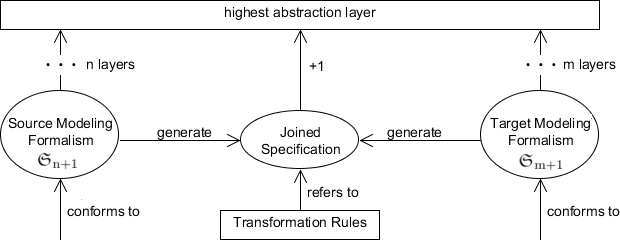
\includegraphics[scale=0.7]{./Figures/simple_modeling_formalism.png}
	\caption[Simplified joined specification]
	{A simplified joined modeling formalism that transformation rules refers to.}
	\label{fig:simple_modeling_formalism}
\end{figure}

Figure~\ref{fig:simple_modeling_formalism} explains that we create a joined
specification from a source modeling formalism and a target modeling formalism
from some abstraction layers. The joined specification is created independent of
the two abstraction layers and is referred to when creating transformation rules
in the DPF Transformation Editor. 

%----------------------------------------------------------------------------------------
% SECTION 2
%----------------------------------------------------------------------------------------

\section{Test case with the DPF Transformation Editor}

\section{Comparison with other editor tools}

In this section we provide a comparison between the three model
transformation environments that we worked with including the DPF Transformation
Editor. In our solution we expanded the Henshin model transformation environment
to be able to apply model transformations to a multi-layered meta-modeling
environment like we discussed in section~\ref{evaluate_solution}. It is natural
that the DPF Transformation Editor will have similarities to the Henshin environment
since our solutions builds heavily on this environment. But we can still
compare our solution with both Henshin and other transformation tools.
Table~\ref{tab:comparing} provides an overview of the DPF Transformation Editor
and the three other model transformation environments that we compared in
section~\ref{tools}. We will consider only some of these elements since some of
them will be explained in later subsections. 

\begin{table}[ht]
\renewcommand*\arraystretch{1.2}
\centering
\begin{tabular}{| c | c | c | c | c |}
\hline
& AGG & Henshin & ATL & DPF Transform \\
\hline
Endogenous transformation & $\surd$ & $\surd$ & $\surd$ & \textcolor{red}{\textbf{---}}\\

Exogenous transformation & $\surd$ & $\surd$ & $\surd$ & $\surd$\\

Input Elements & 1\ldots n & 1\ldots n & 1\ldots n & 1\ldots n\\

Output Elements & 1\ldots n & 1\ldots n & 1\ldots n & 1\ldots n\\

Graphical syntax & $\surd$ & $\surd$ & \textcolor{red}{\textbf{---}} & $\surd$
\\

Meta-modeling layers & 2 & 2 & 2 & $\infty$ \\

Separate meta-models & \textcolor{red}{\textbf{---}} &  $\surd$ &  $\surd$ &  $\surd$ \\

Integrated with EMF & \textcolor{red}{\textbf{---}} & $\surd$ & $\surd$ & $\surd$ \\ 

Supports Java & $\surd$ & $\surd$ & $\surd$ & $\surd$ \\ 

Model transformation file size & 200 kb & 80 kb & 4 kb & 265 kb\\

In-place/out-place transformations & in-place &
in-place & out-place  & out-place \\

\hline
\end{tabular}
\caption{Comparing model transformation tools.}
\label{tab:comparing}
\end{table} 

All four tools supports for an arbitrary number of both input and
output elements. This means that if the tool takes a number of input models, then it
produces the same number of target models. Take an ATL module as an example. It
accepts a fixed number of models as input, and returns a fixed number of target
models. This means that an ATL module can not generate an unknown number of
target models. If there is one input model, then there will be one output model
that conforms to a target meta-model.

Both AGG, DPF Transformation Editor and Henshin provides a graphical syntax to
specify the transformation rules that is potentially intuitive. This is not the
case for ATL, which uses a textual based approach. For ATL the users have to
implement transformation rules in programming code.

The tools can be integrated with Java. For ATL the files containing the
transformation rules have to be created before they can be used in a java
application. In ATL this has to be a ``atl'' file containing a ATL module that
has a list of rules. This is because the ATL transformation engine relies on a
file extension with the name ``atl''. Both Henshin and AGG provides an API that
can be used to create transformation rules, application conditions, type graph,
source graph, etc. The DPF Transformation Editor is quite different since it
utilize the convenience methods that the Henshin API provides. It is possible to
specify transformation rules in the DPF Transformation Editor by implementation
code, but the method to generate Henshin rules requires a single production that
has a left, a right and a common subgraph. We explained what a production was in
section~\ref{Chapter5}.

We can also se that the size of the transformation rules differ amongst the
tools. The examples that are compared are different exogenous model
transformations. This means that a model transformation for all tools
includes a source and target meta-model and a file containing the transformation
rules. By reading the table we can see that an exogenous model transformation in
the DPF Transformation Editor uses 265 kb of the storage space. This number is
so unbelievable small that it will never be noticed in any modern computers.
But there is one interesting thing however, that the transformation rules
defined in ATL is over 60 times smaller than the DPF Transformation Editor.
What this basically means is that creating model transformations through the
use of textual concrete syntax is less space consuming than through the use of
graphical syntax. This is only logical since the graphical syntax based
transformation languages requires more storage space simply because they use
graphical elements to represent the transformation rules.

\subsection{Editing Transformation Rules}

In the DPF Transformation Editor we present the transformation rules in a list of
transformation rules. Each transformation rule is extended with a simplified
version of the DPF Model Editor and a toolbar that contains modeling elements
from a source and a target meta-model. With these modeling elements we can
create and structure a searching pattern and a replacement pattern for each
transformation rules. It is logical that the searching pattern and replacement
pattern create modeling elements that corresponds to the source and target
meta-model, since this is an exogenous model transformation between two
different modeling languages. In Henshin we can choose to create transformation
rules in either the tree based Henshin Model Editor or in a graph based editor.
The DPF Transformation Editor that we created provides an integrated view on
transformation rules, similar to Henshin and GReAT. This means that
we do not provide separate editors to implicitly edit the LHS and the RHS
graphs for a transformation rule like for example AGG does. This is convenient
since editing is now separated in a left hand and a right hand side editor. AGG
can also include a third editing window, that specifies application conditions
for the rule. At first glance AGG will most likely provide a more intuitive
approach to editing transformation rules compared to the integrated view that
Henshin and our solution provides. The users needs to understand the principles
behind graph transformations when working with either tools, but AGG might
present a more intuitive approach since the tool has a clear procedure on how
to create and manage new application rules. However, AGG, Henshin and DPF
Transformation Editor provides a graph based approach to model transformations
even though they introduce different approaches to define transformation rules.
The graphical editor that AGG and Henshin provides are different in such a way
that the creation of rules are different. Both Henshin and AGG has a tree based
editor, but the editor works differently amongst the two tools, see
figure~\ref{fig:AGGTreeBasedEditor} and~\ref{fig:Henshin_TreeEditor} for the
two editors. The graphical editor for our solution is very similar to Henshin,
but does not provide any three based editor. However, when generating to
Henshin transformation rule it is possible to use the tree based editor and
browse through the Henshin rules and application conditions. Keep in mind that
changes done to the Henshin rules might jeopardize the execution of the
transformation rules for DPF specifications.

The third transformation tool we encountered in our comparison is the ATLAS
Transformation Language. And while this tool is definitely not as intuitive as
the the graph transformation tools, once you understand how to create
transformation rules and how to work with the included meta-models, it is a
good framework for working with model transformations. However, if a user do
not fully understand the Object Constraint Language (OCL), ATL is rather a hard
tool to work with. Because OCL has a very leveled learning curve, since it is a
declarative programming language. We are more confident in working with
imperative programming languages during our studies here in Bergen. ATL
provides an editor where the users can use OCL to create and modify
transformation rules. ATL has a very strict way of writing transformation
rules, since the tool uses a textual based approach to create transformation
rules. The user has to use the predefined stereotypes defined by ATL.

\subsection{Meta-modeling}

Meta-models are initialised and handled differently amongst the four tools.
The initialisation of the meta-models for Henshin and ATL is similar. Both of
these tools use Ecore to create meta-models, since they are both integrated with
EMF. For Henshin and ATL the user has to create one Ecore model for both the
source and the target meta-model. Both of these meta-models can be imported both
into Henshin and ATL. One thing that is convenient with Henshin that ATL does
not provide, is that Henshin provides a list of meta-models that is available
for the user. These are meta-models that can be used either as source or target
meta-model. If we want to translate a instance model to an Ecore model, we can
in Henshin import this Ecore meta-model from a list and use it as the target
meta-model.

AGG on the other hand uses a disjoint meta-model. This means that in AGG there
is something called a type graph, and in this type graph both the target and
the source meta-model are defined. AGG handles consistency similar to
Henshin. AGG will restrict the user to only create nodes or arrows between
nodes that are specified in the type graph. Figure \ref{fig:AggTypeGraph}
in chapter 3 shows that there are created references between two meta-models. And
through the use of these references, AGG can create and modify application
rules to translate these two models represented in the type graph. 

Through defining the abstract syntax is where our editor has its biggest
advantage, since the three transformation tools that we worked with utilizes a
two layered approach to modeling. First we create the abstract syntax through a
meta-model and second we specify the concrete syntax through a instance model
of this abstract syntax. This is also implicitly true for the DPF Transformation
Editor, since every DPF specification, regardless of abstraction layer is
represented as an instance model of a DPF specification one abstraction layer
higher. There are some similarities to how we present meta-models like ATL and
Henshin does for the transformation rules and that is through the Ecore model.
There is one major difference however, and that is that our Ecore model is
static and ATL and Henshin's meta-models are dynamic. And by dynamic we mean
that the source meta-model and target meta-model represents the abstract syntax
of some arbitrary modeling language. For the DPF Transformation Editor the
source and target meta-model always corresponds to the same Ecore model and that
is the common meta-model for all specifications. But with the help of
application conditions in Henshin we can define an abstract syntax that the
transformation rules can refer for an unlimited hierarchy layer of
meta-modeling. to can adapt the Henshin transformation language to make it
possible to apply model transformations to a modeling language that is
specified through an unlimited hierarchy layer of meta-modeling. So one could
say that every DPF specification is an instance of a common modeling language
while the abstract syntax for the modeling elements for this DPF specification
are described by another DPF specification one abstraction layer higher.

\subsection{Transformation Rules}
We have seen that the creation of transformation rules varies over the three
different tools. ATL provides a textual based approach and therefore requires
multiple lines of code. The abstract syntax for the three different tools are
not that different, since both Henshin and ATL utilizes the Ecore model to
create meta-models and AGG creates one type graph that contains the abstract
syntax for both the source and target model. The abstract syntax can be
visualized either by using the tree based model editor that EMF provides or by
using a tird party tool for a graphical representation of the models. The
concrete syntax are obviously different between the three tools. AGG and Henshin
provides a concrete graphical syntax, while ATL on the other side provides a
concrete textual syntax for creating and modifying transformation rules. For
both AGG and Henshin the rules can be created and modified by using a graphical
editor. AGG separates the RHS and the LHS in two separate editing parts while
Henshin use predefined word sequences to distinguish the two different sides.
If the rules are quite large, with multiple nodes and arrows the rules
presented in Henshin becomes easier to read and maintain. But both AGG and
Henshin has a clear way of representing the rules and possible attached
application conditions. All three tools have a left hand side
and a right hand side, but are represented differently amongst the rules.
Henshin and AGG use graph patterns to represent the LHS and the RHS while ATL
utilizes logical expressions. In section 3 we discussed that ATL can have both
declarative and imperative transformation rules. In Henshin and AGG the LHS and
the RHS are represented as graphs. Where the LHS represents the pattern graph
that is matched for an instance model and the RHS represents the part that should be
replaced for the instance model. For ATL the LHS represents the source model
while the RHS represents the target model. 

Both AGG and Henshin can specify both negative and positive application
conditions. These are attached to pattern graph or the LHS of a rule. These
application conditions provides a true or false clause that can be used to
restrict the pattern graph. For ATL these conditions are handled by OCL
expressions, where one example is the if-then clause.

\subsection{Rule Scheduling}

ATL does the scheduling implicit, where the user has no control over the
scheduling algorithm defined by the tool. The user can however influence the scheduling
algorithm defined by the ATL transformation engine by designing the logic in the
transformation rules to apply in a certain order. The transformation
engine will first execute the declarative rules before applying the imperative
section of a transformation rule. AGG and Henshin does however, give the
users the possibility to influence how the transformation rules are applied. 
In Henshin and AGG this is handled explicitly before applying the transformation
rules, where the user can change the execution order of the rule.
For example the rules can be applied non-deterministic or in sequential order.To
force the transformation in a sequential order could result in performance
issues compared to applying the rules non-deterministically. AGG provides the
users with the possibility to organize the transformation process into several
phases or layers. These layers are numbered from 0 \ldots n, and the lower the
number the higher the priority for the rule, when it is translated. This gives
the users the possibility to execute rules layer by layer. In Henshin these
rule scheduling mechanisms are referred to as transformation units. For this
tool it is possible to specify units that supports rule iteration, both by
looping through rules until there are no more changes detected or by iterating
through rules for a fixed number of iterations. In Henshin it is also possible
to specify an amalgamation unit, that is an unit that provides a
forall-operation for the matching pattern graph. This unit has a kernel rule
and multiple underlying rules that are matched as often as possible. It is
clear that Henshin provides the users with quite an variety of controlling the
execution of rules.

The DPF Transformation Editor does not provide the user with any control
regarding how to locate matches and how transformation rules are applied. We generate a
Henshin module that contains a set of transformation rules. We can manipulate
the execution order of these transformation rules, but the algorithm that
Henshin uses to locate matching patterns in a source model is part of the
internal infrastructure of Henshin and cannot be manipulated. We can however
force the transformation rules to be executed in a given order. This version of
the Editor has no support defining a schedule mechanism that specifies how the
rules are applied and will for now only run the transformation rules
sequentially. We can decide the priority of the rules by changing the order
that they appear in the DPF Transformation Editor, but this list will apply rules in
sequential order. Most of the transformation tools open to the public provides
solutions to manipulate the scheduling mechanism, for example ATL provides the
users the possibility to define rules as lazy rules and control how they are
applied. While AGG and the Henshin environment lets the users specify the
scheduling mechanism over a few predefined choices. 

Another thing that is special about our integration of Henshin is that locating
matches are handled differently. An application condition is initially meant to
restrict a transformation rule when locating matches. If application conditions
are not specified for a transformation rule in some 2 layered meta-modeling
transformation tool we will still locate a matching pattern that correspond to
modeling elements that are described in the abstract syntax. The application
condition has a vital role in our integration of Henshin, because the
application conditions are checked against the DPF model that are one
abstraction level higher. Without this application condition we would simply get
a target DPF model that has a list of nodes and arrows that conform to the
highest level of abstraction in DPF. The highest level of abstraction in DPF
is always a node and an arrow, that conforms to itself. So while a 2 layered
meta-modeling transformation tool would find matches in a source model that
correspond to the meta-model, the DPF Transformation Editor would find matches to
the linguistic meta-model and not the ontological meta-model at some level of
abstraction. One could state that an application condition for a 2 layered
meta-modeling transformation tool is independent of the transformation rules
while our version the transformation rules are dependent on the application
conditions to be able to produce a correct target model. 

\subsection{Rule Organization}

ATL organizes the transformation rules inside modules, and its therefore easy to
reuse these modules if applicable. This is convenient for
users of ATL since this means that all created rules can be used to form new
transformation rules. Henshin provides the user with the possibility to nest or 
reuse rules in different scheduling mechanism or transformation units
as we discussed in the last paragraph. But Henshin and therefore the DPF
Transformation Editor does however not provide the user with the possibility to
reuse rules in the creation of new rules like in ATL. 

\subsection{Source - Target Relationship}

The DPF Transformation Editor explicitly performs an out-place model
transformation. This means that we create a target model that is independent of
the source model. For all matching modeling elements we locate in the source
model we create in a target model. We then make sure to specify all the nodes
and arrows with its corresponding type from a specification that is located one
abstraction layer higher. AGG does this differently, since the source and target
model are the same model. Matches are located in the source model, while the
target model is updated in the same model. For an exogenous model transformation
it is required that ATL produce the target model in a separate file. Henshin on
the other hand provides in-place model transformations on the source model. But
when we invoke the Henshin interpreter engine programmatically we can check for
changes before and after exeuting a set of transformation rules. Henshin
transformation engine requires a set of transformation rules, and a graph that
contains the source model. This graph contains a list of all the modeling
elements that are part of the source model. This is why we can explicitly make a
model transformation out-place, by checking this list before and after the
transformation and adding translated elements to a target model. The interpreter
will locate matches in the source model through this graph and produce target
elements to this graph. 

For an exogenous transformation in ATL it is mandatory to create a new target
that holds all the target model elements. Exogenous model transformation in ATL
is therefore called an out-place transformations. In AGG on the other hand both
source and target model is always the same model. This means that AGG performs an
in-place update on its original source model. Henshin is a bit more special,
because implicitly it performs in-place update on the source model. But in
Henshin you can initialize variables that explicitly captures the transformed
target elements and save these to a separate file in your storage unit. Note
however, that this can only be done when utilizing the Henshin interpreter
programmatically. 

\subsection{Directionality}

To provide a graph based model transformation with the possibility to translate
in both directions is not a simple task. Because then the tool will have to
provide arbitrary switching between source and target models, and therefore the
pattern and replacement graphs will have to be changed when they are switched.
This means that the LHS and the RHS part of a transformation rules have to be
switched out. This is not provided in the DPF Transformation Editor. One could do
this in two steps, to first locate matches in a source model and produce a
target model and then do another model transformation where the source and
target part is switched. Both Henshin and AGG does not provide this since the
corresponding RHS and LHS graphs are created according to the abstract syntax of
the source and target model. 

Its obvious that all four tools are unidirectional, since they can be
executed in one direction only. That is to compute a target model from a
source model. The tools requires two model transformations to be able to
transform in multiple directions. Where the source and target model and
meta-models switch places. But this is not how multidirectional transformations
work. A multidirectional transformation can execute in both direction when
performing a model transformation.

\subsection{Tracing}

Tracing in the four tools provides an unique link between a source and a target.
The source represents the matched part while the target represents the
generated or replacement part. All three tools provides dedicated support for
traceability. But these traceable links are handled differently amongst the
tools. For ATL the trace model works as a storage location and automatically
creates trace links between source and target elements. These traceable links
are internally used by the ATL transformation engine when executing a model
transformation. But we explained in section 3 that these trace links can be
explicitly captured by creating transformation rules that generates a
collection of trace links in a separate trace file. Henshin does this
differently, because tracing is controlled by the users. Henshin has a
dedicated Trace Model that can be imported to the Henshin module as an Ecore
model. The trace model in Henshin are automatically created when executing
rules, but the user have to manually assign the traceable links inside the
transformation rules. The traces in Henshin are translated when a rule is
executed, and therefore the user has to be aware of this when using these
traces in other rules, since this could lead to the creation of multiple
traceable links between the same elements. The DPF Transformation Editor defines
a traceable link with source and target modeling elements differently amongst
nodes and arrows. For DPF models nodes and arrows are defined by the EClass
modeling element that Ecore provides. Tracing in AGG plays a vital role to
executing model transformations. Traceable elements are created similar to any
other elements when initializing the type graph. With traceable links between
the source and the target elements, AGG can be certain that elements are
transformed. The traceable link in AGG ensures that a match in the pattern
graph is only matched once. If we do not create a traceable link between source
and target elements in AGG, the rules will be applied an endless amount of
times. Tracing amongst the three different tools are different in such a way
that it is required for exogenous model transformations for AGG and ATL. In ATL
the traceable links are created automatically and cannot be controlled by the
users, while in AGG the traceable links are created as bridges between source
and target elements. For Henshin the Trace model is optional.

\subsection{Translating the instance model}

When ATL transformation language executes the application rules for the model to
model transformation, a new model instance is created for the target model. This
means that the source model is independent of the target model. Where Henshin
and AGG performs in-place model to model transformations. This means that they
both operate on an instance model of the source meta-model, and translates
inside this instance model. On the other side, for ATL this is not needed, since
both the source and target model are kept as separated files. This is also
possible to achieve with Henshin. If the user programmatically invoke the
Henshin Interpreter the target model can be forced to be saved in a newly
created file. Henshin will still do an in-place model transformation, but it is
possible to save the translated object in a separate file. It is then possible
to perform an in-place transformation in Henshin while saving the target
instance model in a separate file. The DPF Transformation Editor utilize the
strengths of Henshin to perform an in-place model transformation of a source
model and explicitly creates a target model based on the results of this source
model. All four approaches can however give the same result. Inn AGG and Henshin
the users just need to make sure to delete unwanted elements from the
translated host graph. This is different in the DPF Transformation Editor
since we produce a target graph structure for each matching graph structure and
specifies the target graph structures in a separate target model. 

